% !TeX encoding = UTF-8
% !TeX program = xelatex
% !TeX spellcheck = en_US

\documentclass[degree=doctor,fontset=windows]{ustcthesis}
% degree      = doctor | master | bachelor
% degree-type = academic | professional
% language    = chinese | english
% fontset     = windows | mac | ubuntu | fandol

% \usepackage{multirow,makecell,booktabs}
\usepackage[caption=false, font=footnotesize]{subfig}
% 加载宏包、全部的配置
% !TeX root = ./main.tex

\ustcsetup{
  title              = {布隆过滤器及其衍生数据结构\\在隐私保护协议中的应用},
  title*             = {An example of thesis template for University of Science
                        and Technology of China v\ustcthesisversion},
  author             = {柳枫},
  author*            = {Liu Feng},
  speciality         = {网络空间安全},
  speciality*        = {Mathematics and Applied Mathematics},
  supervisor         = {薛开平教授},
  supervisor*        = {Prof. XXX, Prof. XXX},
  date               = {2024-10-10},
  % date               = {2017-05-01},  % 默认为今日
  % professional-type  = {专业学位类型},
  % professional-type* = {Professional degree type},
  % department         = {数学科学学院},  % 院系,本科生需要填写
  % student-id         = {PB11001000},  % 学号,本科生需要填写
  % secret-level       = {秘密},     % 绝密|机密|秘密|控阅,注释本行则公开
  % secret-level*      = {Secret},  % Top secret | Highly secret | Secret
  % secret-year        = {10},      % 保密/控阅期限
  % reviewer           = true,      % 声明页显示“评审专家签名”
  %
  % 数学字体
  % math-style         = GB,  % 可选:GB, TeX, ISO
  math-font          = xits,  % 可选:stix, xits, libertinus
}


% 加载宏包

% 定理类环境宏包
\usepackage{amsthm}

% 插图
\usepackage{graphicx}

% 三线表
\usepackage{booktabs}

% 表注
\usepackage{threeparttable}

% 跨页表格
\usepackage{longtable}

% 算法
\usepackage[ruled,linesnumbered]{algorithm2e}

% SI 量和单位
\usepackage{siunitx}

% 参考文献使用 BibTeX + natbib 宏包
% 顺序编码制
\usepackage[sort]{natbib}
\bibliographystyle{ustcthesis-numerical}

% 著者-出版年制
% \usepackage{natbib}
% \bibliographystyle{ustcthesis-authoryear}

% 本科生参考文献的著录格式
% \usepackage[sort]{natbib}
% \bibliographystyle{ustcthesis-bachelor}

% 参考文献使用 BibLaTeX 宏包
% \usepackage[style=ustcthesis-numeric]{biblatex}
% \usepackage[bibstyle=ustcthesis-numeric,citestyle=ustcthesis-inline]{biblatex}
% \usepackage[style=ustcthesis-authoryear]{biblatex}
% \usepackage[style=ustcthesis-bachelor]{biblatex}
% 声明 BibLaTeX 的数据库
% \addbibresource{bib/ustc.bib}

% 配置图片的默认目录
\graphicspath{{figures/}}

% 数学命令
\makeatletter
\newcommand\dif{%  % 微分符号
  \mathop{}\!%
  \ifustc@math@style@TeX
    d%
  \else
    \mathrm{d}%
  \fi
}
\makeatother
\newcommand\eu{{\symup{e}}}
\newcommand\iu{{\symup{i}}}

% 用于写文档的命令
\DeclareRobustCommand\cs[1]{\texttt{\char`\\#1}}
\DeclareRobustCommand\env[1]{\texttt{#1}}
\DeclareRobustCommand\pkg[1]{\textsf{#1}}
\DeclareRobustCommand\file[1]{\nolinkurl{#1}}

% hyperref 宏包在最后调用
\usepackage{hyperref}



\begin{document}

\maketitle
% \copyrightpage

\frontmatter
% % !TeX root = ../main.tex

\ustcsetup{
  keywords  = {学位论文, 摘要, 关键词},
  keywords* = {dissertation, abstract, keywords},
}

\begin{abstract}
  摘要分中文和英文两种,中文在前,英文在后,博士论文中文摘要一般 800~1500 个汉字,硕士论文中文摘要一般 500~1000 个汉字。
  英文摘要的篇幅参照中文摘要。

  关键词另起一行并隔行排列于摘要下方,左顶格,中文关键词间空一字或用分号“,”隔开,英文关键词之间用逗号“,”或分号“;”隔开。

  中文摘要是论文内容的总结概括,应简要说明论文的研究目的、基本研究内容、研究方法或过程、结果和结论,突出论文的创新之处。
  摘要应具有独立性和自明性,即不用阅读全文,就能获得论文必要的信息。
  摘要中不宜使用公式、图表,不引用文献。

  中文关键词是为了文献标引工作从论文中选取出来用以表示全文主题内容信息的单词和术语,一般 3~8 个词,要求能够准确概括论文的核心内容。
\end{abstract}

\begin{abstract*}
  This is a sample document of USTC thesis \LaTeX{} template for bachelor,
  master and doctor. The template is created by zepinglee and seisman, which
  orignate from the template created by ywg. The template meets the
  equirements of USTC thesis writing standards.

  This document will show the usage of basic commands provided by \LaTeX{} and
  some features provided by the template. For more information, please refer to
  the template document ustcthesis.pdf.
\end{abstract*}

\tableofcontents
% \listoffigures
% \listoftables
% % !TeX root = ../main.tex

\begin{notation}

  \begin{notationlist}{2em}
    \item[$\displaystyle a$] The number of angels per unit area
    \item[$\displaystyle N$] The number of angels per needle point
    \item[$\displaystyle A$] The area of the needle point
    \item[$\displaystyle \sigma$] The total mass of angels per unit area
    \item[$\displaystyle m$] The mass of one angel
    \item[$\displaystyle \sum_{i=1}^n a_i$] The sum of $a_i$
  \end{notationlist}

\end{notation}



% 也可以使用 nomencl 宏包

% \printnomenclature

% \nomenclature{$\displaystyle a$}{The number of angels per unit are}
% \nomenclature{$\displaystyle N$}{The number of angels per needle point}
% \nomenclature{$\displaystyle A$}{The area of the needle point}
% \nomenclature{$\displaystyle \sigma$}{The total mass of angels per unit area}
% \nomenclature{$\displaystyle m$}{The mass of one angel}
% \nomenclature{$\displaystyle \sum_{i=1}^n a_i$}{The sum of $a_i$}


\mainmatter
% !Tex root = ../main.tex

\chapter{简介}

\section{布隆过滤器}

在构造网络安全相关协议时,我们经常会使用到许多不同类型的数据结构。
其中,布隆过滤器(Bloom filter)~\cite{bloom1970space}作为一种经典的概率型数据结构,在IP地址过滤、识别恶意邮件、DoS 和 DDos 攻击检测等场景有着广泛的应用~\cite{geravand2013bloom}。
% 可搜索加密、隐私信息检索、隐私集合运算等安全协议中有着广泛的应用~\cite{geravand2013bloom}。
% 布隆过滤器的定义是一种空间效率
布隆过滤器是由 $k$ 个哈希函数构造的数组结构,它的作用是快速判断元素是否属于某一集合(membership query),具有空间效率高、判断速度快的特点。
布隆过滤器的结构如图~\ref{fig:Bloom_example}~所示,数组中每个位置上存储的是 $0/1$ 比特,每个元素对应的位置由 $k$ 个哈希函数所确定。
% 它主要有构造和判断元素两个过程。
\begin{figure}[ht]
  \centering
  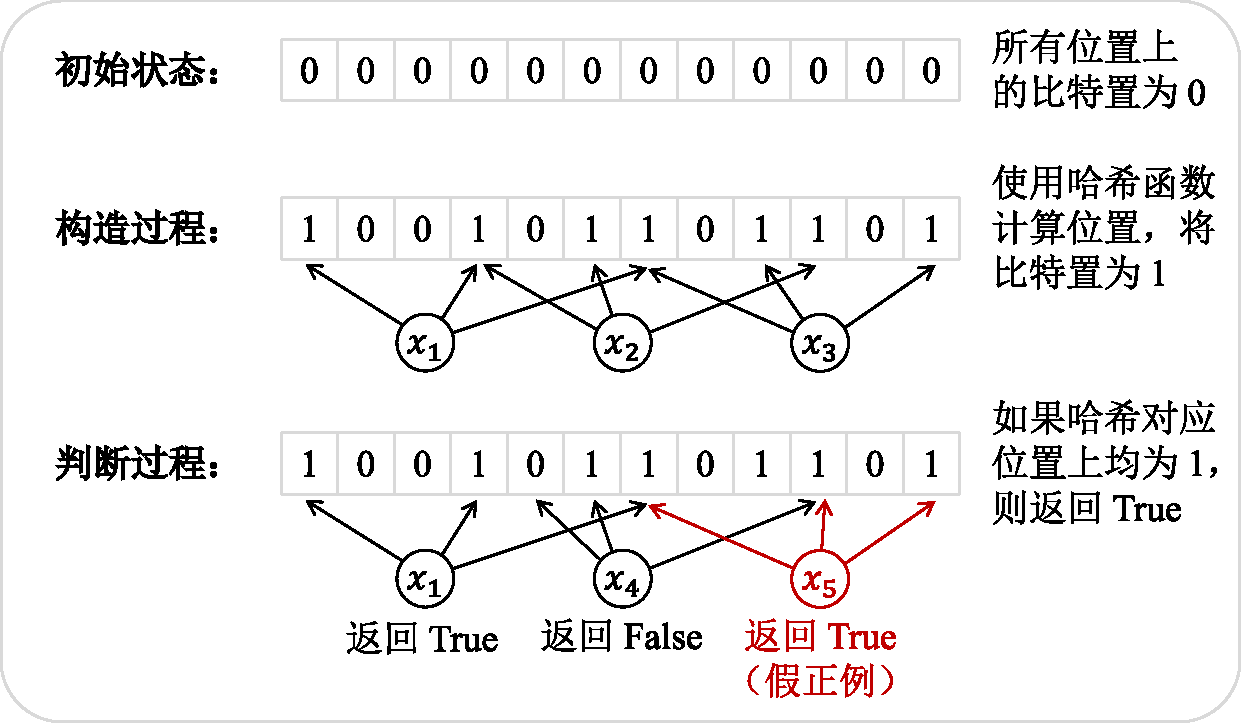
\includegraphics[width=0.9\textwidth]{figures/bf_exp.pdf}
  \caption{布隆过滤器示例($k=3$)}
  \label{fig:Bloom_example}
\end{figure}
以包含 $n$ 个元素的集合 $S=\{x_1, x_2, \dots, x_n\}$ 为例,假设构造的布隆过滤器长度为 $m$,使用的哈希函数为 $\{h_1, h_2, \dots, h_k\}$,其中每个哈希函数 $h_i:\{0,1\}^* \to [1, m]$ 为任意长度的输入到布隆过滤器上某一特定位置的映射。
首先我们将布隆过滤器 $m$ 个位置上的比特都置为 $0$,然后插入集合 $S$ 中的每一个元素。
在插入元素 $x$ 时,需要使用 $k$ 个哈希函数计算出 $k$ 个位置信息,即 $\{h_1(x),h_2(x),\dots, h_k(x)\}$。
最后将布隆过滤器上这 $k$ 个位置上的比特都置为 $1$。
% 一个包含 $n$ 个元素的集合,
在判断某个元素是否属于集合 $S$ 时,只需要计算该元素对应的 $k$ 个位置,然后检查这 $k$ 个位置上的比特是否都为 $1$。
只要有一个位置上出现了 $0$,那么判断结果就是不属于;否则,布隆过滤器认为该元素属于集合 $S$。
对于大小为 $n$ 的集合,其对应的的布隆过滤器需要 $O(nk)$ 的存储开销以及 $O(k)$ 的判断复杂度。

% 布隆过滤器是一种用于快速判断元素是否存在于某一集合的数据结构,它具有空间效率高、判断速度快的特点。
% 但是布隆过滤器也并不是
% 布隆过滤器的构造如图~\ref{fig:Bloom_example}~所示,它是使用 $k$ 个哈希函数 $\{h_1,\dots, h_k\}$ 构造的哈希表结构。
% 在初始状态,哈希表中所有所有位置上的比特都置为 $0$。
% 在构造过程中,对于每个在集合 $S$ 中的元素 $x$,只需要通过 $k$ 个哈希函数计算出对应的位置,并将这些位置上的比特置为 $1$。
% 首先使用这 $k$ 个哈希函数计算出 $k$ 个位置,然后对过滤器中该位置上的比特置为 $1$。
% 对于需要插入的元素,只需要通过 $k$ 个哈希函数计算出对应的位置,并将这些位置上的比特置为 $1$。
% 以大小为 $n$ 的集合 $S$ 为例,对应的布隆过滤器构造需要 $O(nk)$ 的存储开销以及 $O(k)$ 的判断复杂度。

% 布隆过滤器上分为插入(Insert)和查找(Lookup)两个算法,
% 在判断某个元素是否属于集合 $S$ 时,只需要通过哈希函数计算该元素的 $k$ 个位置,然后检查过滤器上这 $k$ 个位置上的比特是否全为 $1$。
% 如果是,返回 True,否则返回 False。
% 从布隆过滤器的构造可以看出,
% 假定有一个集合 $S$,其大小 $|S| = n$,
% 文献\cite{luo2019optimizing}:

% 布隆过滤器(Bloom filter,BF)是一种空间效率高的概率型数据结构,它可以用来快速判断元素是否属于某一集合。
% 布隆过滤器是由 0-1 比特组成的比特向量结构,包含插入(Insert)和查找(Lookup)两个基本算法。
% 以包含 $n$ 个元素的集合 $S=\{x_1, x_2, \dots, x_n\}$ 为例,假设构造的布隆过滤器长度为 $m$,使用的哈希函数为 $\{h_1, h_2, \dots, h_k\}$,其中每个哈希函数 $h_i:\{0,1\}^* \to [0, m-1]$ 为任意长度的输入到布隆过滤器上某一位置的映射。
% 首先我们将布隆过滤器 $m$ 个位置上的比特都置为 $0$,然后再插入集合 $S$ 中的每一个元素。
% 在插入元素 $x$ 时,需要使用 $k$ 个哈希函数计算出 $k$ 个位置信息,即 $\{h_1(x),h_2(x),\dots, h_k(x)\}$。
% 再将布隆过滤器上这 $k$ 个位置上的比特都置为 $1$。
% 一个包含 $n$ 个元素的集合,
% 在判断某个元素是否属于集合 $S$ 时,只需要计算该元素对应的 $k$ 个位置,然后检查这 $k$ 个位置上的比特是否都为 $1$。
% 只要有一个位置上出现了 $0$,那么判断结果就是不属于;否则,布隆过滤器认为该元素属于集合 $S$。

从布隆过滤器的构造和判断过程可以看出,如果一个元素属于集合 $S$,那么判断结果一定是正确的;但是如果一个元素不属于集合 $S$ (如图~\ref{fig:Bloom_example}~中的 $x_5$),布隆过滤器也有可能会认为该元素属于 $S$(输出结果为 True),此时判断错误的概率也称为假正例率(false positive rate)。
尽管布隆过滤器存在误判的问题,但在实际应用场景中,只要将误判率控制在较小的值,一般认为以一定的误判换取低空间开销和高效判断是值得的。

布隆过滤器的假正例率 $\epsilon$ 由布隆过滤器的长度 $m$,使用的哈希函数个数 $k$ 和集合中的元素个数 $n$ 所决定。
根据文献~\cite{luo2019optimizing}中的推导,理论上,误判率 $\epsilon$ 与它们的关系如公式~\eqref{eq:BF_FPR}~所示:
\begin{equation}
    \epsilon = \left[ 1 - \left( 1 - \frac{1}{m} \right)^{nk} \right]^k \approx \left(1 - e^{-\frac{kn}m{}}\right)^k.
    \label{eq:BF_FPR}
\end{equation}
其中,$(1-1/m)^{nk}$ 近似成 $e^{-kn/m}$ 的形式。
为了尽可能降低误判率 $\epsilon$,那么就需要尽可能降低 $e^{-kn/m}$ 的值,这样一来,$k$ 的最优取值为:
\begin{equation}
    k_{opt}= \frac{m}{n}\ln 2 \approx \frac{9m}{13n}.
    \label{eq:BF_k}
\end{equation}
% 即 $m\approx 1.44 \cdot n \cdot k$
此时,误判率大约为 $\epsilon \approx 2^{-k}\approx 0.6185^{m/n}$,过滤器的长度 $m\approx 1.44n\log_2{(1/\epsilon)}$。
通常在实际应用中的误判率要比理论分析上的更高,也有一些工作~\cite{bose2008falsepositive,christensen2010new}对误判率做了更精确的刻画。
% 从式~\ref{eq:BF_k}中可以推出,
布隆过滤器的优势主要体现在以下几个方面:
% 高效性主要体现在两个方面:
\begin{itemize}
    \item \textbf{较低的存储开销:}布隆过滤器的大小与元素本身的大小无关,只与集合中元素的数量有关。比如,当给定 $m$ 与 $n$ 的比值为 $5$ 时,根据公式~\eqref{eq:BF_k} 可以计算出需要的哈希函数数量为 $3$ 或 $4$。因为布隆过滤器中每个位置上存储的都是 $0/1$ 比特,所以过滤器存储大小也就是 $m$ 比特。
    \item \textbf{较高的判断效率:} 因为只需要检查 $k$ 个位置上的比特是否全为 $1$,所以检查一个元素的时间复杂度为 $O(k)$,与集合中元素的数量无关。相比于树形结构的查询复杂度$O(\log(n))$或列表结构的查询复杂度$O(n)$都要更低,尤其当元素数量较多的情况下优势更为明显。
    % 而对于具体的布隆过滤器实例来说,$k$ 的值在初始化阶段就是常数,因此插入和查询的复杂度都为 $O(1)$。
    \item \textbf{不会漏判:} 尽管布隆过滤器在查询时会存在误判的情况,但是它不会出现漏判(假负例)的情况。也就是只要是布隆过滤器判断元素 $x$ 不属于 $S$,那么该论断一定是正确的。
\end{itemize}
% 布隆过滤器的挑战性问题:
但是,布隆过滤器也存在一些局限性:
\begin{itemize}
    \item \textbf{假正例率与过滤器长度:} 由于布隆过滤器中存在假正例的情况,而假正例率与过滤器的长度 $m$ 成反比。根据式~\ref{eq:BF_FPR},二者之间的关系为 $m\approx \frac{13}{9}nk \approx 1.44n\log_2(1/\epsilon)$。为了保证足够低的假正例率,就需要更大的 $m$ 来避免不同哈希映射导致的冲突。如此一来,过滤器的空间利用率就会降低。
    \item \textbf{动态性:} 布隆过滤器本身不支持元素的删除,因为如果是简单将需要删除元素所对应位置的比特置为 $0$,那么就会影响对其他元素的判断。
    \item \textbf{功能性:} 布隆过滤器只能判断元素是否属于某个集合,并不支持检索功能。
    % 能检索元素对应的某一函数值或映射结果。
    % \item 实现,实际实现中需要考虑访问的优化,哈希计算的优化
    % \item 灵活性,哈希函数不能变,集合一开始就是确定的
    % \item 功能有限,只能做成员存在性测试
\end{itemize}

% 布隆过滤器本身是不支持删除的,因为如果是简单将需要删除元素所对应位置的比特置为 $0$,那么就会对其他元素的判断造成影响。
% 降低误判率的方法(思路):首先,

\section{定义及分类}\label{sec:defi_cate}

在介绍布隆过滤器衍生的新型数据结构之前,我们需要对所介绍的数据结构进行分类。
为此,我们首先对这些数据结构进行统一的定义。

\begin{definition}[过滤器]\label{def:filter}
    令 $\mathcal{U}$ 表示元素的集合,$\mathcal{H}$ 为哈希函数的集合。过滤器一般包含以下两个算法:
    % 的插入和查询算法如下所示。
    \begin{itemize}
    \item[$\circ$] $\mathsf{Construct}(S, \mathcal{H}) \to F/\perp$:输入集合 $S \subseteq \mathcal{U}$ 和预先给定的哈希函数集合 $\mathcal{H}$,输出构造的过滤器 $F$(或者以可忽略的概率输出错误指示符 $\perp$)。
    \item[$\circ$] $\mathsf{Evaluate}(x, \mathcal{H}, F) \to \mbox{True}/\mbox{False} $:输入元素 $x$,预先给定的哈希函数集合 $\mathcal{H}$,输出结果 True 或者 False。
    \end{itemize}

    \textbf{正确性:} 对于任意的 $S \subseteq \mathcal{U}$,都有:a).构建过程中,输出 $\perp$ 的概率是可忽略的;b).如果 $F \gets \mathsf{Construct}(S, \mathcal{H})$,且 $F \neq \perp$,那么在判断过程中,对于任意的 $x \in S$,$\Pr[\mathsf{Evaluate}(x, \mathcal{H}, F) = \mbox{True}] = 1$ 始终成立;对于任意 $x' \notin S$,概率 $\Pr[\mathsf{Evaluate}(x', \mathcal{H}, F) = \mbox{True}]$ 为可忽略不计的。
\end{definition}
从以上定义中可以看出,如果一个元素在原本输入的集合中,那么过滤器在判断过程中一定能返回正确的结果,即过滤器中不存在假负例的情况;反之,如果一个元素不存在于输入的集合中,过滤器会大概率返回正确的结果,即过滤器中会以极小的概率出现假正例。

在判断过程中,需要使用 $\mathcal{H}$ 中的哈希函数计算出元素在 $F$ 中对应的位置,再对这些位置上记录的结果进行计算,最后根据计算结果与事先定义的 $f(x)$ 进行比较返回 $\mbox{Ture}$ 或者 $\mbox{False}$。
计算过程也被称为探测(probing),根据探测方式可以将过滤器分为以下三种类型~\cite{dillinger2021ribbon}:
\begin{itemize}
    \item \textbf{AND型:}在通过哈希函数计算出的位置中,如果所有位置上结果都与 $f(x)$ 相等,那么就输出 $\mbox{True}$;
    \item \textbf{OR型:}在通过哈希函数计算出的位置中,如果至少有一个位置上的值与 $f(x)$ 相等,那么就输出 $\mbox{True}$,否则输出 $\mbox{False}$。
    % 该类型的过滤器典型代表是布谷鸟过滤器~\cite{fan2014cuckoo},这种构造可以方便
    \item \textbf{XOR 型:}在通过哈希函数计算出的位置中,如果所有位置上值的异或结果与 $f(x)$ 相等,那么就输出 $\mbox{True}$,否则输出 $\mbox{False}$。
\end{itemize}
从以上分类可以看出,布隆过滤器的判断方式属于AND型。
% AND型的典型代表是布隆过滤器,
OR型的典型代表是布谷鸟过滤器(cuckoo filter)~\cite{fan2014cuckoo},这种构造的特点是支持元素的动态插入和删除。
XOR型的典型代表是异或过滤器(xor filter)~\cite{fan2014cuckoo},这类过滤器在结构上非常紧凑,具有较高的空间利用率,但受限于构建方式,这类构造通常不支持动态更新。

% 这里引用文献~\cite{2024YinSiJiHeYunSuanZhongDeGuanJianShuJuJieGouYanJiu}
不同的过滤器中对 $f(x)$ 的定义也略有不同。
一般来说分为以下几种情况:
\begin{itemize}
    \item $f(x)$ 为比特 $1$,最典型的是布隆过滤器,即要求 $x$ 对应所有位置上的结果都为 $1$,过滤器才会返回 $\mbox{True}$。
    % ,最典型的是布隆过滤器,即只有当通过哈希计算出的所有位置上都为 $1$,那么返回 $\mathsf{True}$。
    \item $f(x)$ 等于元素 $x$ 本身,典型的是混淆布隆过滤器 (garbled Bloom filter)~\cite{dong2013when},即计算的结果为 $x$,过滤器才会返回 $\mbox{True}$。
    \item $f(x)$ 为 $x$ 的指纹(fingerprint),一般指的是 $x$ 的哈希值,典型代表为布谷鸟过滤器,即当有一个位置上的值与 $x$ 的指纹相同,过滤器才会返回 $\mbox{True}$。
    \item $f(x)$ 为任意函数,典型的是 Bloomier 过滤器~\cite{chazelle2004bloomier},也就是说 $f(x)$ 的形式并不重要,或者说只要满足是 $x$ 一种映射关系即可。
\end{itemize}

从上述分类可以看出,对 $f(x)$ 的定义可以是简单的比特 $1$,也可以是关于 $x$ 的任意一种映射关系。
从另一个角度来看,键值型数据也可以看作是从键到值的映射,这样一来,键值型数据也可以编码成过滤器的形式。
按照这种思路得到的构造称作不经意键值存储(Oblivious Key-Value Store, OKVS)。
与过滤器不同,不经意键值存储返回的不是 $\mbox{True}$ 或者 $\mbox{False}$,而是与输入键相对应的值。
% 利用这种思路构造的结构称作不经意的键值存储(Oblivious Key-Value Store, OKVS),与过滤器不同,OKVS 返回的不是 $\mathsf{True}$ 或者 $\mathsf{False}$,而是与输入对应的数值。
不经意键值存储的定义如下:

\begin{definition}[不经意键值存储]\label{def:okvs}
    令 $\mathcal{K}$ 和 $\mathcal{V}$ 分别表示键和值的集合。不经意键值存储包含两个算法:
    \begin{itemize}
        \item[$\circ$] $\mathsf{Encode}(\{(x_1, y_1), (x_2, y_2), \dots, (x_n, y_n)\})$:输入一组键值对 $\{(x_i, y_i)\}_{i\in [1,n]}\subseteq \mathcal{K} \times \mathcal{V}$,输出编码结果 $D$ 或以可忽略的概率输出错误指示符 $\perp$。
        \item[$\circ$] $\mathsf{Decode}(D, k)$:输入编码结果 $D$ 和键 $k\in \mathcal{K}$,输出值 $v\in \mathcal{V}$。
    \end{itemize}

    \textbf{正确性:} 对于任意键值对集合 $A\subseteq \mathcal{K}\times \mathcal{V}$,如果 $\mathsf{Encode}(A) = D$ 且 $D\neq \perp$,那么对于任意的 $(k, v) \in A$,都有 $\mathsf{Decode}(D, k) = v$。

    \textbf{不经意性:} 随机给定两个不同的集合 $\mathcal{K}_0 = \{x_1^0, x_2^0, \dots, x_n^0\}$ 和 $\mathcal{K}_1 = \{x_1^1, x_2^1, \dots, x_n^1\}$,再随机构造集合 $\{y_i\}_{i\in [1,n]}\gets \mathcal{V}$,若 $D \neq \perp$,则分布 $\{D | y_i \gets \mathcal{V}, i\in [1,n], \mathsf{Encode}(\{(x_1^0, y_1), (x_2^0, y_2), \dots, (x_n^0, y_n)\})\}$ 与分布 $\{D | y_i \gets \mathcal{V}, i\in [1,n], \mathsf{Encode}(\{(x_1^1, y_1), (x_2^1, y_2), \dots, (x_n^1, y_n)\})\}$ 计算不可区分。

    对于部分安全需求较高的协议,不经意键值存储还需要满足随机性,即:

    \textbf{随机性:} 对于任意的集合 $A = \{(x_i, y_i)\}_{i\in [1,n]} \subseteq \mathcal{K} \times \mathcal{V}$ 和 $x' \notin \{x_1, x_2, \dots, x_n\}$,如果 $\mathsf{Encode}(A) = D$ 且 $D\neq \perp$,则 $\mathsf{Decode}(D, x')$ 的输出与随机选择的 $v\gets \mathcal{V}$ 统计不可区分。
\end{definition}

% 衡量指标:
我们主要关注这些数据结构在存储和计算方面的性能。
% 评估以上数据结构的性能主要考虑存储和计算两个方面,
在存储开销方面,一是要衡量过滤器本身的长度,即 $m$ 的数值,我们一般使用负载因子(load factor) $\alpha = n/m$ 作为评估指标,即 $\alpha$ 越接近 $1$,说明空间利用率越高;二是需要衡量均摊空间开销(amortized space cost),即平均每个元素上在过滤器中所占用的存储空间。
在计算开销方面,我们主要关注构建/判断(或编码/解码)过程的复杂度。
% 基于以上讨论内容,
表~\ref{tab:construct}~对本文中所介绍的过滤器以及不经意键值存储结构进行了总结。
% 接下来我们将对布隆过滤器衍生的数据结构进行详细介绍。
在接下来的章节,我们将对这些新型数据结构的构建方法进行详细介绍。

\begin{table}[ht]
  \centering
  \caption{不同过滤器及相关结构总结}
  \label{tab:construct}
  \begin{tabular}{cccc}
    \toprule
    探测类型 & 名称 &  $f(x)$  & 负载因子 \\
    \midrule
    AND型 & 布隆过滤器 &  $1$ & $0.7k_{opt}^{-1}$  \\
    % \cmidrule(c){1}
    % \midrule
    % \cmidrule(l){1-2}
    OR型 & 布谷鸟过滤器~\cite{fan2014cuckoo} &  $x$ 的指纹值 &  $0.5-0.95$ \\
    % \midrule
    % \cmidrule(l){1-2}
    \multirow{4}*{XOR型} & 异或过滤器~\cite{graf2020xor}  &  $x$ 的指纹值 & $0.81$ \\
    & 二进制引信过滤器~\cite{graf2022binary}  &  $x$ 的指纹值 & $0.88-0.93$ \\
    & 缎带过滤器~\cite{dillinger2021ribbon} & $x$ 的指纹值 & $0.96-0.99$ \\
    % & Bloomier 过滤器 &  $f(x)$ \\
    % & 混淆布隆过滤器  &  $x$ \\
    & 随机带状不经意键值存储~\cite{bienstock2023NearOptimal} &  键 $x$ 对应的值 $y$ & $0.91-0.97$ \\
    \bottomrule
  \end{tabular}
\end{table}

% \begin{table}[ht]
%   \centering
%   \caption{不同过滤器及相关结构总结}
%   \label{tab:construct}
%   \begin{tabular}{cccc}
%     \toprule
%     名称  &  探测类型  &  $f(x)$  & 均摊存储开销 (bits) \\
%     \midrule
%     布隆过滤器  &  AND型  &  $1$ & $1.44\log_2(1/\epsilon)$  \\
%     布谷鸟过滤器  &  OR型  &  $x$ 的指纹值 &  $2\log_2(1/\epsilon)$ \\
%     异或过滤器  &  XOR型  &  $x$ 的指纹值 & $1.23 \log_2(1/\epsilon)$ \\
%     二进制引信过滤器  & XOR型  &  $x$ 的指纹值 & $1.125 \log_2(1/\epsilon)$ \\
%     缎带过滤器 & XOR型 & $x$ 的指纹值 & $1.01 \log_2(1/\epsilon)$ 到 $1.04 \log_2(1/\epsilon)$ \\
%     % Bloomier 过滤器  &  XOR型  &  $f(x)$ & \\
%     % 混淆布隆过滤器  &  XOR型  &  $x$ & \\
%     随机带状不经意键值存储 &  XOR型  &  键 $x$ 对应的值 $y$ & $1.023 \log_2(1/\epsilon)$ \\
%     \bottomrule
%   \end{tabular}
% \end{table}

\section{总结}

布隆过滤器是一种近似成员查询过滤器(approximate membership query filter),即以一定的假正例率回答查询元素是否存在于集合中。
得益于其简洁的构造方式以及高效的判断性能,布隆过滤器的应用场景非常广泛。
除了前面提到的IP地址过滤、识别恶意邮件、DoS 和 DDos 攻击检测等场景之外,布隆过滤器及其衍生的数据结构也常被用于构造隐私保护相关协议~\cite{zhang2024survey}。
% 常用于对元素的存在性测试,在英文语境中,所谓``存在性测试''也被看作一种查询(m)
% 容易理解的构造以及
% 布隆过滤器的应用场景非常广泛,
% 由布隆过滤器衍生的数据结构大致有两个
布隆过滤器自提出后,各种变体形式层出不穷,如计数式布隆过滤器(counting Bloom filter)~\cite{lifan2000summary},压缩布隆过滤器(compressed Bloom filter)~\cite{mitzenmacher2002compressed},$d$-left 计数式布隆过滤器~\cite{bonomi2006improved},块布隆过滤器(blocked Bloom filter)~\cite{putze2009cache}等。
这些变体本质都是在布隆过滤器构造的基础上提出的各种优化,关于这些结构的介绍不属于本文的讨论范畴。
我们主要介绍布隆过滤器衍生出的新型数据结构,包括布谷鸟过滤器、异或过滤器、不经意键值存储等。
我们将在第~\ref{chp:data_structure}~章对这些衍生新型数据结构进行详细介绍。
% 关于这些衍生数据结构我们将在第二章
最后,我们将在第~\ref{chp:application}~章介绍这些数据结构在隐私保护协议上的应用。

% !Tex root = ../main.tex

\chapter{新型数据结构}

在这一章,我们将重点介绍由布隆过滤器衍生出来的几个特殊数据结构,分别是布谷鸟过滤器,异或型过滤器以及不经意的键值存储。
% 从上一章的分类我们知道,对于

\section{布谷鸟过滤器}

从上一章的分类我们可以知道,布谷鸟过滤器是一种 OR 型的过滤器,且 $f(x)$ 为 $x$ 的指纹信息。
布谷鸟过滤器的概念最早是由 Fan 等人~\cite{fan2014cuckoo} 于2014年提出的,其构造方式受到了布谷鸟哈希表(Cuckoo Hash Table)~\cite{pagh2004cuckoo}的启发。
在介绍布谷鸟过滤器之前,我们首先介绍布谷鸟哈希表的构造。

\subsection{布谷鸟哈希表}

布谷鸟哈希表可以看作一个由多个桶(bucket)组成的数组结构。
对于每个元素 $x$ 来说,它在哈希表中对应两个候选位置,分别由两个哈希函数 $h_1(x)$ 和 $h_2(x)$ 决定。
在插入元素 $x$ 时,首先检查 $x$ 对应的两个位置上的桶中是否有多余位置。
如果两个桶都有多余空间,则直接将 $x$ 放入桶中;如果两个桶都已满,则随机在一个候选位置上踢出一个元素并将 $x$ 放入该位置上。踢出的元素则重新插入到它对应的另一个候选位置上。
如图所示,假设每个桶中都只能存储一个元素,当插入元素 $x$ 时,首先计算出它的两个候选位置分别是 $2$ 和 $6$。
因为 $2$ 和 $6$ 两个位置都已满,这里选择踢出位置 $6$ 上的元素 $a$,并将 $x$ 放入其中。
被踢出的 $a$ 则重新插入到它的另一个候选位置,也就是 $4$ 上。
由于位置 $4$ 上已有元素 $c$,则把 $c$ 踢出,将 $a$ 存储在位置 $4$ 中,并将 $c$ 重新插入到它的候选位置 $1$ 上,最终结果如图所示。
这种``踢出-插入''的思路与布谷鸟下蛋时会将蛋放入其他鸟的巢穴,并挤出原本巢中蛋的行为很相似,因此而得名。

\subsection{布谷鸟过滤器的构造}

与布谷鸟哈希表类似,布谷鸟过滤器也是由多个桶组成的数组结构。
不同的是,在布谷鸟过滤器中每个桶中存储的并不是元素本身,而是元素的指纹。
这就导致在将桶中的元素指纹踢出时,无法根据指纹信息确定它的另一个候选位置。
因此布谷鸟过滤器采用了部分密钥布谷鸟哈希(partial-key cuckoo hashing)的技巧来解决该问题。
也就是将元素的两个候选位置与元素的指纹值建立联系,这样就能在只知道元素的指纹值和其中一个位置信息的情况下计算出另一个位置信息。
具体来说,对于元素 $x$,其对应的两个候选位置计算如下:
\begin{align}
  h_1(x) & = \mathsf{hash}(x) \\
  h_2(x) & = h_1(x) \oplus \mathsf{hash}(x\mbox{'s fingerprint}) \label{eq:cuckoo_h2}
\end{align}
式~\ref{eq:cuckoo_h2}中的异或操作正好满足了上述性质,即$h_1(x)$ 也可以通过 $h_2(x)$ 和 $x$ 的指纹信息计算得出。
另外,在异或操作中采用的是$x$指纹的哈希而不是$x$的指纹本身,这样做是因为如果只用指纹本身的话,两个候选位置之间的距离就受限于指纹的取值范围。
比如使用 $8$ 比特长度的指纹,那么两个候选位置之间最多相差 $256$。
而使用指纹的哈希则可以确保两个候选位置可以分布在过滤器中的任意位置,从而降低哈希碰撞的概率并提高存储空间的利用率。

\subsection{布谷鸟过滤器的性能}



\section{异或型过滤器}


\section{不经意的键值存储}


% !Tex root = ../main.tex

\chapter{在隐私保护上的应用}

\section{在可搜索加密方面的应用}

\section{在隐私信息检索方面的应用}

\section{在隐私集合计算方面的应用}

% % !TeX root = ../main.tex

\chapter{简介}

\section{一级节标题}

\subsection{二级节标题}

\subsubsection{三级节标题}

\paragraph{四级节标题}

\subparagraph{五级节标题}

本模板 \pkg{ustcthesis} 是中国科学技术大学本科生和研究生学位论文的 \LaTeX{}
模板, 按照《中国科学技术大学研究生学位论文撰写手册》(最近在修订中,以下简称《撰写手册》)和
《\href{https://www.teach.ustc.edu.cn/?attachment_id=13867}
{中国科学技术大学本科毕业论文(设计)格式}》的要求编写。

Lorem ipsum dolor sit amet, consectetur adipiscing elit, sed do eiusmod tempor
incididunt ut labore et dolore magna aliqua.
Ut enim ad minim veniam, quis nostrud exercitation ullamco laboris nisi ut
aliquip ex ea commodo consequat.
Duis aute irure dolor in reprehenderit in voluptate velit esse cillum dolore eu
fugiat nulla pariatur.
Excepteur sint occaecat cupidatat non proident, sunt in culpa qui officia
deserunt mollit anim id est laborum.



\section{脚注}

Lorem ipsum dolor sit amet, consectetur adipiscing elit, sed do eiusmod tempor
incididunt ut labore et dolore magna aliqua.
\footnote{Ut enim ad minim veniam, quis nostrud exercitation ullamco laboris
  nisi ut aliquip ex ea commodo consequat.
  Duis aute irure dolor in reprehenderit in voluptate velit esse cillum dolore
  eu fugiat nulla pariatur.}

% % !TeX root = ../main.tex

\chapter{浮动体}

\section{三线表}

三线表是《撰写手册》推荐使用的格式,如表~\ref{tab:exampletable}。

\begin{table}
  \centering
  \caption{表号和表题在表的正上方}
  \label{tab:exampletable}
  \begin{tabular}{cl}
    \toprule
    类型   & 描述                                       \\
    \midrule
    挂线表 & 挂线表也称系统表、组织表,用于表现系统结构 \\
    无线表 & 无线表一般用于设备配置单、技术参数列表等   \\
    卡线表 & 卡线表有完全表,不完全表和三线表三种       \\
    \bottomrule
  \end{tabular}
\end{table}

如果有表注,推荐使用 \pkg{threeparttable}。这样可以与表格对齐,满足部分评审老师的要求。

\begin{table}
  \centering
  \begin{threeparttable}
    \caption{带表注的表格}
    \label{tab:tablewithnotes}
    \begin{tabular}{cl}
      \toprule
      类型   & 描述                                       \\
      \midrule
      挂线表 & 挂线表也称系统表、组织表,用于表现系统结构 \\
      无线表 & 无线表一般用于设备配置单、技术参数列表等   \\
      卡线表 & 卡线表有完全表,不完全表和三线表三种       \\
      \bottomrule
    \end{tabular}
    \begin{tablenotes}[flushleft]
      \item 注:表注分两种,第一种是对全表的注释,用不加阿拉伯数字排在表的下边,
      前面加“注:”;第二种是和表内的某处文字或数字相呼应的注,
      在表里面用带圈的阿拉伯数字在右上角标出,然后在表下面用同样的圈码注出来
    \end{tablenotes}
  \end{threeparttable}
\end{table}

编制表格应简单明了,表达一致,明晰易懂,表文呼应、内容一致。
排版时表格字号略小,或变换字体,尽量不分页,尽量不跨节。
表格太大需要转页时,需要在续表上方注明“续表”,表头页应重复排出。



\section{插图}

有的同学可能听说“\LaTeX{} 只能使用 eps 格式的图片”,甚至把 jpg 格式转为 eps。
事实上,这种做法已经过时。
而且每次编译时都要要调用外部工具解析 eps,导致降低编译速度。
所以我们推荐矢量图直接使用 pdf 格式,位图使用 jpeg 或 png 格式。

\begin{figure}[ht]
  \centering
  
\includegraphics[width=0.3\textwidth]{ustc-badge.pdf}
  \caption{图号、图题置于图的下方}
  \label{fig:badge}
  \note{注:图注的内容不宜放到图题中。}
\end{figure}

关于图片的并排,推荐使用较新的 \pkg{subcaption} 宏包,
不建议使用 \pkg{subfigure} 或 \pkg{subfig} 等宏包。



\section{算法环境}

模板中使用 \pkg{algorithm2e} 宏包实现算法环境。关于该宏包的具体用法,
请阅读宏包的官方文档。

\begin{algorithm}
  \SetAlgoLined
  \KwData{this text}
  \KwResult{how to write algorithm with \LaTeX2e }

  initialization\;
  \While{not at end of this document}{
    read current\;
    \eIf{understand}{
      go to next section\;
      current section becomes this one\;
    }{
      go back to the beginning of current section\;
    }
  }
  \caption{算法示例1}
  \label{algo:algorithm1}
\end{algorithm}

注意,我们可以在论文中插入算法,但是插入大段的代码是愚蠢的。
然而这并不妨碍有的同学选择这么做,对于这些同学,建议用 \pkg{listings} 宏包。

% % !TeX root = ../main.tex

\chapter{数学}

\section{数学符号}

《撰写手册》要求数学符号遵循 GB/T 3102.11—1993《物理科学和技术中使用的数学符号》
\footnote{原 GB 3102.11—1993,自 2017 年 3 月 23 日起,该标准转为推荐性标准。}。
该标准参照采纳 ISO 31-11:1992 \footnote{目前已更新为 ISO 80000-2:2019。},
但是与 \TeX{} 默认的美国数学学会(AMS)的符号习惯有所区别。
具体地来说主要有以下差异:
\begin{enumerate}
  \item 大写希腊字母默认为斜体,如
    \begin{equation*}
      \Gamma \Delta \Theta \Lambda \Xi \Pi \Sigma \Upsilon \Phi \Psi \Omega.
    \end{equation*}
    注意有限增量符号 $\increment$ 固定使用正体,模板提供了 \cs{increment} 命令。
  \item 小于等于号和大于等于号使用倾斜的字形 $\le$、$\ge$。
  \item 积分号使用正体,比如 $\int$、$\oint$。
  \item
    偏微分符号 $\partial$ 使用正体。
  \item
    省略号 \cs{dots} 按照中文的习惯固定居中,比如
    \begin{equation*}
      1, 2, \dots, n \quad 1 + 2 + \dots + n.
    \end{equation*}
  \item
    实部 $\Re$ 和虚部 $\Im$ 的字体使用罗马体。
\end{enumerate}

以上数学符号样式的差异可以在模板中统一设置。
但是还有一些需要用户在写作时进行处理:
\begin{enumerate}
  \item 数学常数和特殊函数名用正体,如
    \begin{equation*}
      \uppi = 3.14\dots; \quad
      \symup{i}^2 = -1; \quad
      \symup{e} = \lim_{n \to \infty} \left( 1 + \frac{1}{n} \right)^n.
    \end{equation*}
  \item 微分号使用正体,比如 $\dif y / \dif x$。
  \item 向量、矩阵和张量用粗斜体(\cs{symbf}),如 $\symbf{x}$、$\symbf{\Sigma}$、$\symbfsf{T}$。
  \item 自然对数用 $\ln x$ 不用 $\log x$。
\end{enumerate}

模板中使用 \pkg{unicode-math} 宏包配置数学字体。
该宏包与传统的 \pkg{amsfonts}、\pkg{amssymb}、\pkg{bm}、
\pkg{mathrsfs}、\pkg{upgreek} 等宏包\emph{不}兼容。
本模板作了处理,用户可以直接使用 \cs{bm}, \cs{mathscr},
\cs{upGamma} 等命令。
关于数学符号更多的用法,参见 \pkg{unicode-math} 宏包的使用说明和符号列表
\pkg{unimath-symbols}。



\section{数学公式}

数学公式可以使用 \env{equation} 和 \env{equation*} 环境。
注意数学公式的引用应前后带括号,建议使用 \cs{eqref} 命令,比如式~\eqref{eq:example}。
\begin{equation}
  \hat{f}(\xi) = \int_{-\infty}^\infty f(x) \eu^{-2 \uppi \iu x \xi} \dif x.
  \label{eq:example}
\end{equation}

多行公式尽可能在“=”处对齐,推荐使用 \env{align} 环境,比如式~\eqref{eq:align_2}。
\begin{align}
  a & = b + c + d + e \label{eq:align_1} \\
    & = f + g. \label{eq:align_2}
\end{align}



\section{量和单位}

量和单位要求严格执行 GB 3100~3102—1993 有关量和单位的规定。
宏包 \pkg{siunitx} 提供了更好的数字和单位支持:
\begin{itemize}
  \item 为了阅读方便,四位以上的整数或小数推荐采用千分空的分节方式:\num{55235367.34623}。
    四位以内的整数可以不加千分空:\num{1256}。
  \item 数值与单位符号间留适当空隙:\SI{25.4}{mm},\SI{5.97e24}{\kilo\gram},
    \SI{-273.15}{\degreeCelsius}。 例外:\SI{12.3}{\degree},\ang{1;2;3}。
  \item 组合单位默认使用 APS 的格式,即相乘的单位之间留一定空隙: \si{kg.m.s^{-2}},
    也可以使用居中的圆点: \si[inter-unit-product = \ensuremath{{}\cdot{}}]{kg.m.s^{-2}}。
    GB 3100—1993 对两者都允许,建议全文统一设置。
  \item 量值范围使用“~”:\SIrange{10}{15}{mol/L}。
  \item 注意:词头 \textmu{} 不能写为 u,如:\si{umol} 应为 \si{\micro\mole}、\si{\umol}。
\end{itemize}



\section{定理和证明}

示例文件中使用 \pkg{amsthm} 宏包配置了定理、引理和证明等环境。
用户也可以使用 \pkg{ntheorem} 宏包。

\begin{definition}
  If the integral of function $f$ is measurable and non-negative, we define
  its (extended) \textbf{Lebesgue integral} by
  \begin{equation}
    \int f = \sup_g \int g,
  \end{equation}
  where the supremum is taken over all measurable functions $g$ such that
  $0 \le g \le f$, and where $g$ is bounded and supported on a set of
  finite measure.
\end{definition}

\begin{assumption}
The communication graph is strongly connected.
\end{assumption}

\begin{example}
  Simple examples of functions on $\mathbb{R}^d$ that are integrable
  (or non-integrable) are given by
  \begin{equation}
    f_a(x) =
    \begin{cases}
      |x|^{-a} & \text{if } |x| \le 1, \\
      0        & \text{if } x > 1.
    \end{cases}
  \end{equation}
  \begin{equation}
    F_a(x) = \frac{1}{1 + |x|^a}, \qquad \text{all } x \in \mathbb{R}^d.
  \end{equation}
  Then $f_a$ is integrable exactly when $a < d$, while $F_a$ is integrable
  exactly when $a > d$.
\end{example}

\begin{lemma}[Fatou]
  Suppose $\{f_n\}$ is a sequence of measurable functions with $f_n \geq 0$.
  If $\lim_{n \to \infty} f_n(x) = f(x)$ for a.e. $x$, then
  \begin{equation}
    \int f \le \liminf_{n \to \infty} \int f_n.
  \end{equation}
\end{lemma}

\begin{remark}
  We do not exclude the cases $\int f = \infty$,
  or $\liminf_{n \to \infty} f_n = \infty$.
\end{remark}

\begin{corollary}
  Suppose $f$ is a non-negative measurable function, and $\{f_n\}$ a sequence
  of non-negative measurable functions with
  $f_n(x) \le f(x)$ and $f_n(x) \to f(x)$ for almost every $x$. Then
  \begin{equation}
    \lim_{n \to \infty} \int f_n = \int f.
  \end{equation}
\end{corollary}

\begin{proposition}
  Suppose $f$ is integrable on $\mathbb{R}^d$. Then for every $\epsilon > 0$:
  \begin{enumerate}
    \renewcommand{\theenumi}{\roman{enumi}}
    \item There exists a set of finite measure $B$ (a ball, for example) such
      that
      \begin{equation}
        \int_{B^c} |f| < \epsilon.
      \end{equation}
    \item There is a $\delta > 0$ such that
      \begin{equation}
        \int_E |f| < \epsilon \qquad \text{whenever } m(E) < \delta.
      \end{equation}
  \end{enumerate}
\end{proposition}

\begin{theorem}
  Suppose $\{f_n\}$ is a sequence of measurable functions such that
  $f_n(x) \to f(x)$ a.e. $x$, as $n$ tends to infinity.
  If $|f_n(x)| \le g(x)$, where $g$ is integrable, then
  \begin{equation}
    \int |f_n - f| \to 0 \qquad \text{as } n \to \infty,
  \end{equation}
  and consequently
  \begin{equation}
    \int f_n \to \int f \qquad \text{as } n \to \infty.
  \end{equation}
\end{theorem}

\begin{proof}
  Trivial.
\end{proof}

\newtheorem*{axiomofchoice}{Axiom of choice}
\begin{axiomofchoice}
  Suppose $E$ is a set and ${E_\alpha}$ is a collection of
  non-empty subsets of $E$. Then there is a function $\alpha
  \mapsto x_\alpha$ (a ``choice function'') such that
  \begin{equation}
    x_\alpha \in E_\alpha,\qquad \text{for all }\alpha.
  \end{equation}
\end{axiomofchoice}

\newtheorem{observation}{Observation}
\begin{observation}
  Suppose a partially ordered set $P$ has the property
  that every chain has an upper bound in $P$. Then the
  set $P$ contains at least one maximal element.
\end{observation}
\begin{proof}[A concise proof]
  Obvious.
\end{proof}

% % !TeX root = ../main.tex

\chapter{引用文献的标注}

模板使用 \pkg{natbib} 宏包来设置参考文献引用的格式,
更多引用方法可以参考该宏包的使用说明。



\section{顺序编码制}

\subsection{角标数字标注法}

\ustcsetup{
  cite-style = super,
}
\noindent
\begin{tabular}{l@{\quad$\Rightarrow$\quad}l}
  \verb|\cite{knuth86a}|         & \cite{knuth86a}         \\
  \verb|\citet{knuth86a}|        & \citet{knuth86a}        \\
  \verb|\cite[42]{knuth86a}|     & \cite[42]{knuth86a}     \\
  \verb|\cite{knuth86a,tlc2}|    & \cite{knuth86a,tlc2}    \\
  \verb|\cite{knuth86a,knuth84}| & \cite{knuth86a,knuth84} \\
\end{tabular}


\subsection{数字标注法}

\ustcsetup{
  cite-style = inline,
}
\noindent
\begin{tabular}{l@{\quad$\Rightarrow$\quad}l}
  \verb|\cite{knuth86a}|         & \cite{knuth86a}         \\
  \verb|\citet{knuth86a}|        & \citet{knuth86a}        \\
  \verb|\cite[42]{knuth86a}|     & \cite[42]{knuth86a}     \\
  \verb|\cite{knuth86a,tlc2}|    & \cite{knuth86a,tlc2}    \\
  \verb|\cite{knuth86a,knuth84}| & \cite{knuth86a,knuth84} \\
\end{tabular}



\section{著者-出版年制标注法}

\ustcsetup{
  cite-style = authoryear,
}
\noindent
\begin{tabular}{l@{\quad$\Rightarrow$\quad}l}
  \verb|\cite{knuth86a}|         & \cite{knuth86a}         \\
  \verb|\citep{knuth86a}|        & \citep{knuth86a}        \\
  \verb|\citet[42]{knuth86a}|    & \citet[42]{knuth86a}    \\
  \verb|\citep[42]{knuth86a}|    & \citep[42]{knuth86a}    \\
  \verb|\cite{knuth86a,tlc2}|    & \cite{knuth86a,tlc2}    \\
  \verb|\cite{knuth86a,knuth84}| & \cite{knuth86a,knuth84} \\
\end{tabular}

\ustcsetup{
  cite-style = super,
}

% 注意,参考文献列表中的每条文献在正文中都要被引用。这里只是为了示例。
\nocite{*}


\bibliography{bib/ref}  % 参考文献使用 BibTeX 编译
% \printbibliography       % 参考文献使用 BibLaTeX 编译

\appendix
% % !TeX root = ../main.tex

\chapter{补充材料}


\section{补充章节}

补充内容。


\backmatter
% % !TeX root = ../main.tex

\begin{acknowledgements}

在研究学习期间,我有幸得到了三位老师的教导,
他们是:我的导师,中国科大XXX研究员,中科院X昆明动物所马老师以及美国犹他大学的XXX老师。
三位深厚的学术功底,严谨的工作态度和敏锐的科学洞察力使我受益良多。
衷心感谢他们多年来给予我的悉心教导和热情帮助。

感谢XXX老师在实验方面的指导以及教授的帮助。
科大的XXX同学和XXX同学参与了部分试验工作,在此深表谢意。

\end{acknowledgements}

% % !TeX root = ../main.tex

\begin{publications}

\section*{已发表论文}

\begin{enumerate}
\item A A A A A A A A A
\item A A A A A A A A A
\item A A A A A A A A A
\end{enumerate}

\section*{待发表论文}

\begin{enumerate}
\item A A A A A A A A A
\item A A A A A A A A A
\item A A A A A A A A A
\end{enumerate}

\section*{研究报告}
\begin{enumerate}
\item A A A A A A A A A
\item A A A A A A A A A
\item A A A A A A A A A
\end{enumerate}

\end{publications}


\end{document}
